\documentclass[tikz,border=10pt]{standalone}

\usepackage{amsmath}
\usepackage{tikz}
\usepackage{hyperref}
\usepackage{tkz-graph}
\usetikzlibrary{arrows}
\usetikzlibrary{petri}

\newcommand*{\rechterWinkel}[3]{% #1 = point, #2 = start angle, #3 = radius
   \draw[shift={(#2:#3)}] (#1) arc[start angle=#2, delta angle=90, radius = #3];
   \fill[shift={(#2+45:#3/2)}] (#1) circle[radius=1.25\pgflinewidth];
}

\begin{document}
	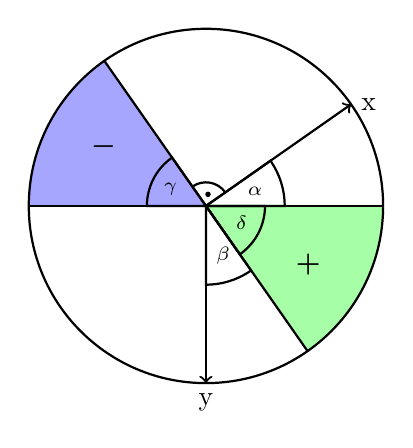
\begin{tikzpicture}[
		-,
		auto,
		node distance=1.6cm,
		thick
	]
	  	
	  	\fill[fill=green!35] (0,0) -- (-55:2.25cm) arc (-55:0:2.25cm) -- cycle;
	  	\fill[fill=blue!35] (0,0) -- (125:2.25cm) arc (125:180:2.25cm) -- cycle;
	  	\draw (0,0) -- (0:1cm) arc (0:35:1cm) -- cycle;
	  	\draw (0,0) -- (-90:1cm) arc (-90:-55:1cm) -- cycle;
	  	\draw (0,0) -- (-55:0.75cm) arc (-55:0:0.75cm) -- cycle;\\
	  	\draw (0,0) -- (180:0.75cm) arc (180:125:0.75cm) -- cycle;
	  	\draw (0,0) circle (2.25cm);
%	  	\draw[->] (-3,0) -- (3,0) node[right] {x};		
%	  	\draw[->] (0,-3) -- (0,3) node[right] {y};	
	  	\draw[->] (0,0) -- (35:2.25cm) node[right] {x};
	  	\draw[->] (0,0) -- (-90:2.25cm) node[below] {y};
	  	\draw (180:2.25cm) -- (0:2.25cm);
	  	\draw (125:2.25cm) -- (-55:2.25cm);
	  	\rechterWinkel{0,0}{35}{0.3}; 
	  	\node at (1.3,-0.75) {$\boldsymbol{+}$};
	  	\node at (-1.3,0.75) {$\boldsymbol{-}$};
	  	\draw (0,0) -- (0:1.25cm) node[above,midway] {\scriptsize{$\alpha$}};
%	  	\draw (0,0) -- (-90:1.25cm) node[above,midway,sloped] {\scriptsize{$\beta$}};
%	  	\draw (0,0) -- (-55:0.9cm) node[above,midway,sloped] {\scriptsize{$\delta$}};
		\draw (0,0) -- (-90:1.25cm) node[right,midway] {\scriptsize{$\beta$}};
	  	\draw (0,0) -- (0:0.9cm) node[below,midway] {\scriptsize{$\delta$}};
	  	\draw (0,0) -- (180:0.9cm) node[above,midway,sloped] {\scriptsize{$\gamma$}};
	\end{tikzpicture}
\end{document}